\documentclass[10pt,letterpaper]{article} % {{{
\usepackage[top=0.85in,left=2.75in,footskip=0.75in]{geometry}
\usepackage{amsmath,amssymb}
% Use adjustwidth environment to exceed column width (see example table in text)
\usepackage{changepage}

% textcomp cpackage and marvosym package for additional characters
\usepackage{textcomp,marvosym}
\usepackage{subcaption}


\usepackage[T1]{fontenc}
\usepackage{lmodern}
% cite package, to clean up citations in the main text. Do not remove.
\usepackage{cite}

% Use nameref to cite supporting information files (see Supporting Information section for more info)
\usepackage{nameref,hyperref}

% line numbers
\usepackage[right]{lineno}

% ligatures disabled
\usepackage[nopatch=eqnum]{microtype}
\DisableLigatures[f]{encoding = *, family = * }

% color can be used to apply background shading to table cells only
\usepackage[table]{xcolor}

% array package and thick rules for tables
\usepackage{array}
\usepackage{caption}
\captionsetup[figure]{labelfont={bf},labelformat={default},labelsep=period,name={Fig}}


% create "+" rule type for thick vertical lines
\newcolumntype{+}{!{\vrule width 2pt}}

% create \thickcline for thick horizontal lines of variable length
\newlength\savedwidth
\newcommand\thickcline[1]{%
  \noalign{\global\savedwidth\arrayrulewidth\global\arrayrulewidth 2pt}%
  \cline{#1}%
  \noalign{\vskip\arrayrulewidth}%
  \noalign{\global\arrayrulewidth\savedwidth}%
}

% \thickhline command for thick horizontal lines that span the table
\newcommand\thickhline{\noalign{\global\savedwidth\arrayrulewidth\global\arrayrulewidth 2pt}%
\hline
\noalign{\global\arrayrulewidth\savedwidth}}


% Remove comment for double spacing
%\usepackage{setspace} 
%\doublespacing

% Text layout
\raggedright
\setlength{\parindent}{0.5cm}
\textwidth 5.25in 
\textheight 8.75in

% Bold the 'Figure #' in the caption and separate it from the title/caption with a period
% Captions will be left justified
\usepackage[aboveskip=1pt,labelfont=bf,labelsep=period,justification=raggedright,singlelinecheck=off]{caption}
\renewcommand{\figurename}{Fig}
\renewcommand{\succ}{\textrm{succ}}

\newcommand{\fref}[1]{Fig~\ref{#1}}
\newcommand{\eref}[1]{Eq~(\ref{#1})}
% Use the PLoS provided BiBTeX style
\bibliographystyle{plos2015}

% Remove brackets from numbering in List of References
\makeatletter
\renewcommand{\@biblabel}[1]{\quad#1.}
\makeatother



% Header and Footer with logo
\usepackage{lastpage,fancyhdr,graphicx}
\usepackage{epstopdf}



\usepackage[english]{babel}
\usepackage{graphicx,helvet}
\usepackage{color}
\usepackage{url}
\usepackage{amssymb}
\usepackage[utf8]{inputenc}
\usepackage{hyperref}
% \usepackage[inline]{showlabels}
\usepackage{bbm,bm}
\usepackage{soul}
\usepackage{amsfonts}

\usepackage{tikz}
\usetikzlibrary{arrows}
\usetikzlibrary{quantikz}

\usepackage[draft,inline,nomargin]{fixme} \fxsetup{theme=color}
\FXRegisterAuthor{cp}{acp}{\color{blue}CP}
\FXRegisterAuthor{tb}{ttb}{\color{green}TB}




%\pagestyle{myheadings}
\pagestyle{fancy}
\fancyhf{}
%\setlength{\headheight}{27.023pt}
\rfoot{\thepage/\pageref{LastPage}}
\renewcommand{\headrulewidth}{0pt}
\renewcommand{\footrule}{\hrule height 2pt \vspace{2mm}}
\fancyheadoffset[L]{2.25in}
\fancyfootoffset[L]{2.25in}
\lfoot{\today}

%% Include all macros below

\newcommand{\lorem}{{\bf LOREM}}
\newcommand{\ipsum}{{\bf IPSUM}}
\DeclareMathOperator{\tr}{tr}
\newtheorem{definition}{Definition}
\newtheorem{theorem}{Theorem}

%% END MACROS SECTION

% }}}
\begin{document}

\section{Simulación de cosas de dos qubits}

En general, un canal de dos qubits va a requerir 4 qubits de ancilla. El circuito para hacerlo es una de las figuras del artículo y es una generalización sencilla del de un qubit.\\

Algunos posibles canales a simular son por ejemplo:
\begin{itemize}
\item $\varepsilon(\rho) = k \rho + (1-k) (\sigma_z \otimes \sigma_z) \rho (\sigma_z \otimes \sigma_z) $.
\item $\varepsilon(\rho) = (1-k_1-k_2) \rho + k_1 (\sigma_z \otimes I) \rho (\sigma_z \otimes I) + k_2 (I \otimes \sigma_z) \rho (I \otimes \sigma_3)$.
\end{itemize}
Como el primer canal solo involucra 2 de los 16 operadores de Pauli, en realidad sólo requiere un qubit de ancilla. El segundo canal requiere 2 qubits de ancilla. \\

Entonces, los dos son fáciles de implementar en las compus cuánticas. 
Por ejemplo, el segundo canal se puede hacer con el siguiente circuito:

\begin{figure}[h!]
\begin{quantikz}
\lstick{$q_0$} & \qw  & \gate{\sigma_3} & \qw & \qw  \\
\lstick{$q_1$} & \qw & \qw & \gate{\sigma_3}  & \qw  \\
\lstick{$\tilde{q}_0$} & \gate[wires=2][3cm]{\quad\quad \text{Crear el estado de dos qubits}\quad\quad} & \octrl{-2} & \ctrl{-1}  & \qw \\
\lstick{$\tilde{q}_1$} & \gateinput{$\;\;\;\;\;\;\; \sqrt{1-k_1-k_2} |0 \rangle |0 \rangle + \sqrt{k_1} |0 \rangle |1 \rangle + \sqrt{k_2} |1 \rangle |0 \rangle $} & \ctrl{-3} & \octrl{-2} & \qw
\end{quantikz}
\end{figure}

Por ejemplo, para unos cuantos puntos dentro de las opciones de $k_1, k_2$ para el segundo canal, se obtienen las siguientes fidelidades:

\begin{figure}[h!]
\begin{center}
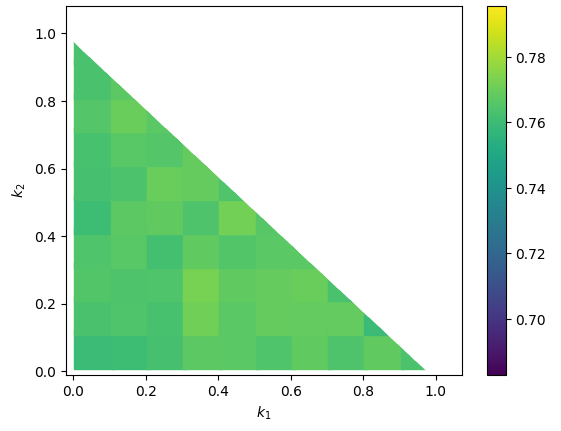
\includegraphics[width=0.5\textwidth]{images/2qbit.png}\\
\caption{Fidelidades para distintas elecciones de $k_1, k_2$ para el segundo canal mostrado arriba.  Al parecer las fidelidades no cambian mucho. }
\end{center}
\end{figure}

\newpage
\section{Ver cómo suben los datos otros artículos similares de Plos One}

Por lo que encontré, muchos de los artículos no tenían datos abiertos al público.
De los pocos que sí, casi todos subían un link a un repositorio de github que  contiene el código que hayan usado y quizá documentos con los resultados de dicho código.\\

Puse lo que pienso que se podría subir en la carpeta "Codigo/Para-subir" en el repositorio. 



\newpage
\section{Revisar la motivación que ponen otras simulaciones cuánticas}

Algunos artículos que encontré y lo que ponen.

Identifico los siguientes temas:
\begin{itemize}
\item[1.] {\color{green} La simulación de sistemas cuánticos es un tema poco explorado y que vale la pena estudiar para entender más de sistemas cuánticos abiertos.}
\item[2.] {\color{blue}  Hacemos la simulación no necesariamente por algo útil, sino que para aprovechar que hay computadoras cuánticas.}
\item[3.] {\color{orange} Porque la simulación cuántica es una de las aplicaciones más prometedoras de la computación cuántica (y una de las aplicaciones que se pensaron inicialmente)}
\end{itemize}

Aquí están los artículos:

\begin{itemize}
\item \textbf{Quantum Simulation of Open Quantum Systems Using Density-Matrix Purification (Anthony W. Schlimgen et al.) PRL
} \\

With the increased
use of quantum algorithms for unitary-gate-based quantum
computers, techniques for casting non-unitary operations into
unitary forms have become increasingly important.


\item  \textbf{Quantum Simulation of Open Quantum Systems Using a Unitary Decomposition of Operators (Anthony W. Schlimgen, et al.) PRL:}


The time evolution of an electronic state is
critical to predicting many important physical phenomena
including exciton transport [1], molecular conductivity [2],
chemical catalysis [3], quantum phase transitions [4, 5], and
magnetization [6]. Often these processes involve non-trivial
interactions with a large environment, requiring the definition and treatment of open quantum systems [7–15]. Recent
research has considered the simulation of open quantum systems on quantum devices [16–20].

\item \textbf{Efficient universal quantum channel simulation in IBM's cloud quantum computer (Shi-Jie Wei, Tao Xin, Gui-Lu long) Science China:}\\ 

Quantum simulation can efficiently simulate the dynamics of diverse systems
[1, 6-10] in condensed matter [11, 12], quantum chemistry
[13], and high-energy physics [14-16], which are intractable
by classical computers. Moreover, every practical quantum
system is open system because of the inevitable coupling to
the environment. {\color{green} Thus, quantum simulation of open system
is an equally important and more general subject to explore.
However, open system quantum simulation is still in the
early stages of development [17-23] and remains largely unexplored. The quantum simulation of open systems promises
powerful applications in a class of physical problems, such as
preparing various special state [24-28], thermalizing in spinboson systems and complex many fermion-boson systems
[29, 30], and studying nonequilibrium dynamics [31].} \\

\item \textbf{Testing quantum computers with the protocl of quantum state matching (Adrian Ortega, Orsolya Kalman) Physica Scripta} \\

The fields of Quantum Computation and Quantum Information have received a huge boost in the last years with
the advent of ‘public’ quantum computation.
{\color{blue} Current devices can be accessed remotely, opening the possibility
for the larger public to carry out experiments and to test them by running programs.} Quantum computers(qcs)
can be based on several different physical systems such as superconducting qubits[1–3], trapped ions[4],
photonic devices[5] and neutral atoms[6]. Given all these possibilities, questions, such as computational
efficiency, error correction capability, stability and computational power start to become important matters for
future applications.\\

\item \textbf{Experimental quantum channel simulation (He Lu et al)}: \\

{ \color{blue} Quantum simulation [1–3] is the most promising near-term
application of quantum computing due to the resource requirements for imitating some classically intractable systems
being significantly less onerous that for other applications
such as factorization.} Experimental quantum simulation on
closed systems is well studied using photons [4], atoms [5]
and trapped ions [6]. Quantum simulation of open-system
dynamics also has variety of applications, such as dissipative quantum phase transitions [7] and dissipative quantumstate engineering [8], thermalization [9], quantum noise generators [10], non-Markovian dynamics [11], and non-unitary
quantum computing [12].

\item \textbf{Quantum Simulation of quantum channels in nuclear magnetic resonance.(Tao Xin, Shi-Jie Wei, Julen S. Pedernales, Enrique Solano and Gui-Lu Long) Physical Review A: }\\

\textbf{En éste artículo hacen algo muy parecido a lo nuestro, pues hacen un algoritmo para simular canales cuánticos. Además, lo usan para Amplitude damping, Phase damping y depolarizing.}\\

In the last decades, significant progress has been achieved in
the isolation and coherent control of quantum systems, allowing for the observation of their unitary dynamics [1–7].
{\color{orange} Such a
degree of controllability has resulted in the implementation of
quantum machines composed of a growing number of qubits,
which have been used for key tests of quantum simulations
and quantum computers. As envisioned by Feynman [8],
large-scale quantum simulators would open the door to the
analysis of new quantum physical phenomena and to the
study of various models that are nowadays intractable with
classical computers.}
{\color{green} In opposition to quantum simulators of
closed quantum systems, the simulation of open quantum
systems, which has also been the subject of some research
both from a theoretical [9–17] and an experimental [18–20]
point of view, has been comparatively less explored. } In this
sense, both from a theoretical and an experimental perspective,
simulating open quantum systems pose relevant challenges.
For example, understanding how quantum systems interact
with their environment could potentially shed light on the
physics of photosynthetic processes or transport phenomena
in general [21,22], which in turn could help us design more
efficient light-harvesting devices [23–25]. It could also help
us understand dissipation and thermalization processes, or
the nature of phase transitions. In the same manner, topics
related to the foundations of quantum physics, such as the measurement process or the quantum-to-classical transition [26],
would greatly benefit from a deeper physical understanding of
open quantum systems. \\



\item \textbf{Simulating noisy quantum channels via quantum state preparation algorithms (Marcelo Zanetti et al):} \\

En este artículo hacen un algoritmo para simular canales cuánticos generales y lo demuestran en las computadoras de IBM. Sin embargo, no hablan mucho de motivación. \\

\item \textbf{Experimental Demonstration of Force Driven Quantum Harmonic Oscillator in IBM
Quantum Computer (Alakesh Baishya et al.)} \\

Quantum simulation is one of the tremendously growing areas in the field of quantum computation which
has significant goals and opportunities. From the
past decades, this powerful area has been applied to
variety of scientific disciplines, e.g., physics2–6, quantum chemistry7,8, quantum biology9,10, and computer
science11 to name a few. Several time-dependent mass
harmonic oscillators including the most famous socalled Caldirola-Kanai oscillator12,13 have been extensively studied over the past years14–17. IBM quantum
experience, has played a considerable role from the recent years, the platform using which a number of research
works have been performed in the field of quantum simulation. These include observation of Uhlmann phase19, chemical isomerization reaction20, simulation of far-fromequilibrium dynamics21, Ising model simulation22, quantum multi-particle tunneling23, quantum scrambling24, and simulation of Klein-Gordon equation25 to name a
few. Other sub-disciplines such as developing quantum
algorithms26–33, testing of quantum information theoretical tasks34–38, quantum cryptography39–42, quantum error correction43–46, quantum applications47–52 have also
been explored.

\item \textbf{Algunos otros art\'iculos que hacen alguna simulaci\'on cu\'antica:}

\begin{itemize}
\item \textbf{Experimental Implementation of Quantum Walks on
IBM Quantum Computers (F. Acasiete et al.)} 


\item  \textbf{Quantum amplitude estimation algorithms on IBM quantum
devices (Pooja Rao et al)}



\item \textbf{Quantum circuit simulation of superchannels (Kai Wang and Dong-Sheng Wang)} \\
\end{itemize}


\item \textbf{Ahora art\'iculos que hacen algo de circuitos cu\'anticos parametrizados y que hablan de optimizar este tipo de circuitos.}


\begin{itemize}
\item  \textbf{Optimizing Parametrized Quantum Circuits
with Free-Axis Single-Qubit Gates (Hiroshi Watanabe)}:\\

Parametrized quantum circuit (PQC) is one of the most essential components of hybrid quantum-classical
algorithms on near-term quantum devices [1–3]. 
The design of PQC is critical in variational quantum algorithms. Oversimplified PQC cannot express
the optimal quantum state even if it could be implemented on noisy quantum devices. On the other
hand, a PQC designed with a deep circuit for high expressibility cannot be implemented on currently available noisy quantum devices.\\

\item  \textbf{Single-qubit rotations in parametrized quantum circuits (S.E. Rasmussen, Loft)}:

En este art\'iculo ven c\'omo optimizar algoritmos cu\'anticos parametrizados reduciendo la cantidad de rotaciones de un qubit.

\end{itemize}







\end{itemize}



\newpage
\section{La definicion de circuito cuantico}

En ningún lugar se define bien qué es un circuito cuántico. Por ejemplo, en wikipedia lo definen así:

In quantum information theory, a quantum circuit is a model for quantum computation, similar to classical circuits, in which a computation is a sequence of quantum gates, measurements, initializations of qubits to known values, and possibly other actions. 

En el Chuang y otros libros, generalmente van entrando de poco en poco y nunca es algo que definan tal cual.


\newpage
\section{Los comentarios}
Los puse también en el documento main, en donde he contestado algunos.


\begin{enumerate}
\item I fail to see the point here - the logic of the paper is: 
1. "open quantum systems can be modeled through a class of channels representing he various types of decoherence." 2. "Quantum circuits are a convenient gate-based formalism that is well understood and has an extensive body of work, and experimentally accessible."
3. We map (generalised) Pauli channels onto quantum circuits, as a way to simulate them.

What I am missing is what do we learn by doing it which cant be learned by actually performing the Pauli channel onto a quantum system? For example, applying well controlled sx, sy, sz operations and their coherent parametric combination using a photonic polarisation or path encoding is experimentally trivial. Why would I need to decompose (not even effectively for any channel) the pauli channels to match a gate based description? Which class of problems can we simulate that cannot be simulated otherwise? Is there any advantage (for example in speed up, resources like ancillas required, resistance to unwanted noise etc..?)

Intuitively, it seems incredibly harder resource wise to create the sum b|gamma> superposition state needed for the ancilla, just for the sake of having it into a "quantum circuit" perspective.

\item Really confusing notation, I suggest use the much more well known relation using the Levi-Civita tensor.

\item At this point I am missing a proper defiition of a "quantum circuit" consistent with the mathematical formalism. The authors start from the very basic regarding Pauli channels, but give for granted the quantum circuit formalism.

\item So another way to see this is that the simulation through the proposed decomposition works only for depolarising channels, and fails otherwise. 

\item I wholeheartedly agree with this statement, and I would go so far as to claim that this is true in general, even at the center of the tethraedron. \\

El statement es: These straightforward channels could be accomplished more efficiently by
simply applying the corresponding Pauli operation directly. \\

\item but this is a severe disadvantage, that begs the question: what is the advantage? \\

\item This definition is vague - given the vagueness of the term "quantum circuit".
 Here what you are defining is just a unitary operation acting on a N-qubit Hilbert space, that is parameter dependent only locally on one specific qubit. 
 
\item again, this is not a conclusion from theorem 1. This is literally Definition 1. Also, use the proper notation here - make A and B operators living on an dim N Hilbert state, and R explixitly dependent on s and operating on qubit N. Then the matrix representation of the operators is a $2^n\times 2^n$ matrix which is applied to the state j....


The explanation in words in not sufficient.

\item true only if the initial j states are normalised, but they were undefined.


\item How can it make sense to define A and B applied respectively to the last 3 and the first qubit?

\item  Please, at least give an example of this semiarbitrary construction of A and B.

\item I don't understand what operatively is happening here. Select the state 0, apply B, apply s, apply A and then "straight forward calculations" lead to what?

\item so this is just the proof that the proposed operative definition of A and B is properly normalised, right?

\item there is literally one parameter in one qubit, of course it depends on one parameter...
 how can this be a result?
  
 \item This is interesting, instead of giving only some random examples, I would actually explore more in details the zoology of this class of dynamical maps - if lucky, you would find class of interesting problems that can be simulated effectively in an experimental setup by just accessing one parameter (as the authors say, just with one set of waveplates, for example), 
 
 \item I feel that there needs to be a treatment of what happens, at least qualitatively at higher than two dimension, as one of the selling point is the generality of the formalism for N qubit. I expect, however, that the higher the dimension, the less rich is the space that can be parametrised by only one parameter, so.. what is the applicability of the theorem for higher dimensions?
 
 \item Imprcise (using parametrized quantum
circuits.)
 
 
 
 \item This reasoning I miss, simplifying for achieving what goal? 
  
 \item There is no quantification of this, it´s not even the focus of the paper 
 
 \item citation required here
\end{enumerate}


\end{document}
